% Chapter Template

\chapter{Mathematical Background} % Main chapter title

\label{chap:Chapter3} % Change to a consecutive number; for referencing this chapter elsewhere, use \ref{chap:Chapter2}

\textcolor{red}{Optimisation approach in vision, "machinery/mechanics", literature review, ill-posed inverse problems.}

Image segmentation falls under the mathemtical classification as being an \textit{ill-posed inverse problem} \citep{Poggio1985,Terzopoulos1986}.
It is an inverse problem since we require a model from the observation, this simply means given the results, what are the causes.
In image segmentation this translates to, given a 2D matrix of intensity values, which pixels belong to the object and which belong to the background.
Image segmentation is also an ill-posed problem since their is a lack of uniqueness or stability of a solution \citep{Kabanikhin2008}, which are two of the three requirements for a solution to be \textit{well-posed}, the other being existence.
Image segmentation is an ill-posed because immense amount of information is suppressed in the acquisition processed \citep{Tarantola2005,Bertero1998,Bertero2006}.
Many tasks in vision are inherently or can be reformulated as ill-posed inverse problems e.g. scene reconstruction, stereo matching, image restoration, image deconvolution, etc.
Computer vision is used heavily in industry, medicine and life science fields included, hence there is a need for robust, enviromentally resistant approach.
The \textit{optimisation approach} is an elegant way to obtain a solution.
In computer vision, a problem can be posed as an optimisation problem as follows: We are given a coarse, discrete and noisy, approximation of the visual data, $d$, we aim to infer some hidden quantities $x$, labels, depth, probable pixel intensty, etc, based on it.
We then have to design an \textit{objective function}, also known as an \textit{energy function} or \textit{cost function},

\begin{equation}
	E:(x,d) \rightarrow \Re,
\end{equation}

which has to be optimised such that the optimsation of the function provides a solution to the problem.
$E(x,d)$ assigns an energy or a cost to each combination $(x,d)$ of the input and hidden quantities.
$E$ provides a measure of goodness to how well the candidate solution $x$ fits the expectation given the data $d$.
In optimisation of this function we seek a minimum energy,

\begin{equation}
	x^{*} = \argmin_{x}E(x,d),
	\label{eq:gibbsenergy}
\end{equation}

which has roots in Statistical Physics where lower energies correspond to more stable solutions.
This gives us a general idea of how we should assign energies to solutions; better a solution, the lower an energy we should assign to it.
In this case, a huge number of inference problems in vision can be solved by minimising the associated energy.
A solution is only as good as the energy model and the optimisation technique. Once a precice energy and minimising algorithm are found, the problem is essentially solved \citep{Delong2011}. 

Early attempts in computer vision would solve problems like these using iteration or relaxation methods \citep{Waltz1975,Rosenfeld1976}.
In these attempts the problems are solved in a Calculus of variations framework, this is still a popular approach to optimisation in vision since Poggio \textit{et al.}. \citep{Poggio1985} proposed an integrated framework to regularisation theory for vision \citep{Sakaue1999}.
Many important advancements in computer vision are proposals for a better energy, a better algorithm or both \citep{Delong2011,Boykov2001,Kolmogorov2005,Mumford1989,Shi1997}.
In this thesis we focus on discrete energy optimisation using graph cuts for image segmentation.

\textcolor{red}{Plan for the chapter.}
Image segmentation falls under a broader catergory of problems known as \textit{labelling problems}.
The aim is to find the best label, foregound/object or background, for each pixel.
In \Cref{sec:LabellingProblems} we briefly discuss labelling problems and its formulation as an energy minimisation problem.

%----------------------------------------------------------------------------------------
%	SECTION 1
%----------------------------------------------------------------------------------------

\section{Labelling Problems}
\label{sec:LabellingProblems}

Among the many computer vision problems, image segmentation is the most easy to understand labelling problem.
A labelling problem is simply assigning, to an observation, a label that most accurately explains it.
An observation can be anything that we wish to classify e.g. pixels, features, salient points, depth measurement, etc.
A label is a description of that observation.
There are two types of labels: \textit{semantic labelling} (person, car, tree, sky, face, eye, etc) or \textit{pixel-wise labelling} (texture, shape, colour, background/object, etc) \citep{Delong2011,Athanasiadis2007}.

To formulate a labelling problem we need a set of \textit{cites}, intuitively known as observations, and a set of \textit{labels}, a set of explanations.
The goal is to find the best explanation given the observations.
In computer vision, the observations, can be features, image segments, etc.
However, they will typically represent pixels in an image with some natual structure or ordering.
Let 

\begin{equation*}
	\mathcal{P} = \{1, 2, \ldots, n\}
\end{equation*}

be the set of $n$ cites and 

\begin{equation*}
\mathcal{L} = \{l_1, l_2, \ldots, l_k\}
\end{equation*}

be the set of $k$ labels.
A discrete labelling is a map $f: \mathcal{P} \rightarrow \mathcal{L}$ that assigns each discrete variable $f_p$ one value from $\mathcal{L}$ and $f=\{f_p\}_{p \in \mathcal{P}}$ which is known as a \textit{configuration}.
We are interested in binary segmentation, also known as \textit{binarization}, which implies we have two explanations in our label set, $k=2$.
The labels of interest are the \textit{background} and the \textit{object}.
Although the solution space is finite, it is very large and grows exponentially as the image size increases or as the number of labels increases.
The number of possible configurations is given by $|\mathcal{L}|^{|\mathcal{P}|}$.
Table \ref{tab:configuration} shows the largeness of the solution space even for very small images and a few labels.
In pratice, the image sizes used in Table \ref{tab:configuration} is too small, hence finding a solution is not easy.
Most often, settling for an approximate solution is "good enough".

\def\arraystretch{1.2}
\begin{table}[ht]
	\caption{The impact of the number of cites and labels on the solution space}
	\label{tab:configuration}
	\begin{tabular}{|c|c|c|c|}
		\hline 
		Image ($\mathcal{P}$) & Number of cites ($|\mathcal{P}|$) & Number of labes ($|\mathcal{L}|$) & Number of configurations $|\mathcal{L}|^{|\mathcal{P}|}$ \\ 
		\hline 
		$64 \times 64$ & $2^{12}=4096$ & $2$ & $2^{2^{12}} = 2^{4096}=n$ \\
		\hline 
		$128 \times 128$ & $2^{14}=16384$ & $2$ & $2^{2^{14}} = 2^{16384} = n^4$ \\ 
		\hline 
		$64 \times 64$ & $2^{12}=4096$ & $3$ & $3^{2^{12}} = 3^{4096} \approx n^{1.585}$ \\ 
		\hline 
	\end{tabular}
\end{table}
 

%----------------------------------------------------------------------------------------
%	SECTION 2
%----------------------------------------------------------------------------------------

\section{Maximum A Posteriori Estimation for Discrete Models}
\label{sec:MAPEstimates}

As previously mentioned, image segmentation is can be viewed as a labelling problem.
The problem is the huge search space in which the solution exists, or possibly more than one.
We need a metric that is able to appropriately weight a configuration $f$.
\textit{Random Fields} are able to provide a structured and yet flexible probabilistic framework for labelling problems.
\textit{Markov Random Fields} (MRFs) and \textit{Conditional Random Fields} (CRFs) are mostly used in vision tasks.
We focus on the discrete image representation provided by MRFs in which we can embed the properties of a desired segmentation solution.
MRFs are pivotal in designing, weighting and structuring graphs, so we give a brief introduction into the concepts needed to understand the probabilistic make-up for graph cut image segmentation.

%----------------------------------------------------------------------------------------
%	SUBSECTION 1
%----------------------------------------------------------------------------------------

\subsection{Markov Random Fields}
\label{sec:MarkovRandomFields}

A \textit{random field} (RF) is a stochastic process where each random variable is indexed by a spatial variable \citep{Adler2007,Gikhman1996}.
A random field model can be intuitively represented as an undirected graph $\mathcal{G}(\mathcal{V}_{RF},\mathcal{E}_{RF})$ where $\mathcal{V_{RF}} = \{1, \ldots, n\}$ is the set of sites which correspond to a random variable for each pixel in $\mathcal{P}$, $\mathcal{E}_{RF}$ is the set of undirected edges which links the random variables.
In vision, random variables which correspond to neighbouring or nearby pixels are linked.
These links model interdependency and in images, nearby pixels exhibit a high degree of spatial correlation (similarity) \citep{Brett2003}.
Common connectivity arrangements in 2D images are 4- and 8-connectivity.
Similarly, higher dimensional data can be represented using graph.
For 3D images, common connectivity arrangements are 6- and 26-connectivity.
Connectedness is illustrated in \autoref{fig:connectedness} for 4-connectivity for 2D image data and 6-connectivity for 3D image data.
In this thesis we are concerned with 2D images only.
Two sites, $p$ and $q$, are neighbours if edge $(p,q) \bigcup (q,p) \in \mathcal{E}_{RF}$.
The set of neighbours of $p$ are denoted $\mathcal{N}_p$.
The RF associated with $\mathcal{P}$ is denoted as $\mathbf{Y} = \{Y_p:p \in \mathcal{P}\}$, where each $Y_p$ can be assigned one of $k$ labels from $\mathcal{L}$.
A 4-connected RF is illustrated in \autoref{fig:randomfield}.
A \textit{clique} $c$ is a fully connected subgraph; it is defined as $\forall p,q \in c, p \in \mathcal{N}_q$ and $q \in \mathcal{N}_p$.
In a clique, each site is connected to all other sites.

The joint event $\{Y_1=y_1, \ldots, Y_n=y_n\}$ where $y_p \in \mathcal{L}$ in called a \textit{realisation} or \textit{configuration} for the random field $\mathbf{Y}$.
For readability we simplify the joint event notation to $\mathbf{Y}=\mathbf{y}$ where $\mathbf{y}=\{y_p : p \in \mathcal{P}\}$.
The image segmentation problem is now in the form of an inference problem where the image $\mathbf{x}$ is the observation of a hidden random field $\mathbf{Y}$ and the solution is given by the \textit{maximum a posteriori} (MAP), i.e. the solution is given by

\begin{equation}
	\mathbf{y^*} = \argmax_{\mathbf{y} \in \mathcal{Y}}\Pr(\mathbf{y}|\mathbf{x}),
	\label{eq:mrfprobability}
\end{equation}

where $\mathcal{Y}$ denotes the set of all possible labellings. $\mathbf{Y}$ is said to be a \textit{Markov random field} (MRF) if:

\begin{align}
	&\Pr(\mathbf{Y}=y) > 0&  &\forall y \in \mathbf{Y},& &(Positivity),&\\
	&\Pr(Y_p=y_p | x_{\mathcal{P}\setminus \{p\}}) = \Pr(Y_p=y_p | y_{\mathcal{N}_p})&  &\forall p \in \mathcal{P},& &(Markovianity),&
\end{align}

The positivity property constrains all configurations to have non-zero probability and is needed to ensure that the joint probability can be uniquely determined by the local conditional probabilities \citep{Smith1997}.
The Markovinatity property states that a site is conditionally independant of all other sites given it's neighbours.

MRFs are on of the most popular probabilistic modelling tools and was introduced to the computer vision community by Geman and Geman \citep{Geman1984} and Besag \citep{Besag1986}.
MRFs allow us to model local contextual constraints, such as spatial interactions between pixels.
According to Baye's rule, the posterior probability relation is:

\begin{equation}
	\Pr(\mathbf{y}|\mathbf{x}) \propto \Pr(\mathbf{x}|\mathbf{y})\Pr(\mathbf{y}),
\end{equation}

$\Pr(\mathbf{x}|\mathbf{y})$ encapsulates the depenency ofthe labels on the observation, it is the likelihood of observing $\mathbf{x}$ given $\mathbf{y}$.
$\Pr(\mathbf{y})$ is the probability of that specific labelling among all labellings $\mathcal{Y}$.
The joint distribution can be specified as a \textit{Gibbs Random Field} (GRF) \citep{Lafferty2001,HammersleyClifford1971}:

\begin{equation}
	\Pr(x|y) = \frac{1}{Z}\prod_{c \in \mathcal{C}}\exp(-\Psi_c(\mathbf{x}_c)),
	\label{eq:gibbs1}
\end{equation}

where $\mathcal{C}$ is the set of cliques.
\autoref{fig:n4} shows a simple MRF construction.
This MRF contains cliques of order one and two, i.e. $\mathcal{C} = \{1, 2, \ldots, 9, \{1,2\}, \{1,4\}, \ldots, \{8,9\}\}$. \autoref{fig:n8} shows a more densely connected MRF where there are cliques of order one, two and three, i.e. $\mathcal{C} = \{1, 2, \ldots, 9, \{1,2\}, \{1,4\}, \{1,5\}, \ldots, \{5,9\}, \{8,9\}, \{1,2,5\}, \{2,3,5\}, \ldots, \{5,6,9\} \}$.
However, cliques of orders higher than two are ignored for computational reasons.
In \autoref{eq:gibbs1} the term $\Psi_c(\mathbf{x}_c)$ is known as a \textit{potential function} for the clique $c$, where $\mathbf{x}_c = \{x_i, i \in c\}$.
The constant $Z$ is called the \textit{partition function} and ensures that the sum of all probabilities is one.
After expanding \autoref{eq:gibbs1} for a maximum clique order of two, the conditional distribution of a pairwise MRF is:

\begin{equation}
\Pr(x|y) = \frac{1}{Z}\prod_{i \in \mathcal{V}}\exp(-\Psi_i(x_i))\prod_{(i,j) \in \mathcal{E}}\exp(-\Psi_{ij}(x_i,x_j)),
\label{eq:gibbs2}
\end{equation}

where $\mathcal{V} = \{1,2,\ldots,n\}$ and $\mathcal{E}$ is the set of pairwise edges, $\Psi_i$ is the unary potential function, for first order cliques, and $\Psi_{ij}$ is the pairwise potential function, for second order cliques.

\begin{figure}[!t]
	\centering
	\subfigure[]
	{
		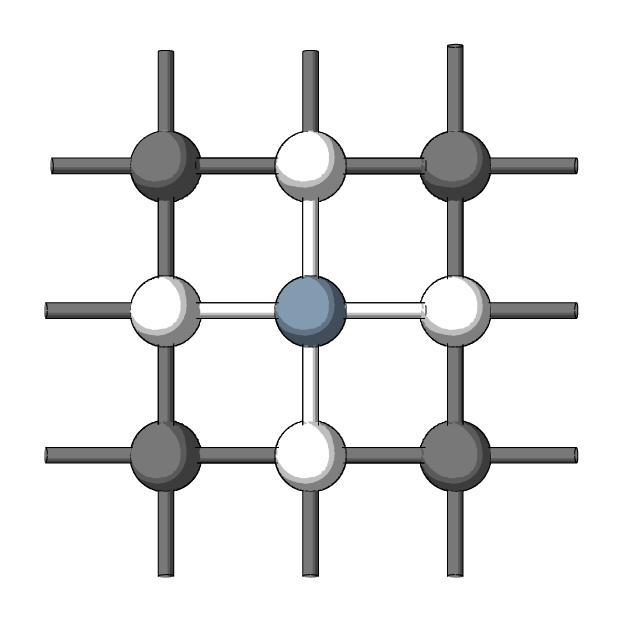
\includegraphics[width=0.48\columnwidth]{2dn4_lattice.png}
		\label{fig:lattice2dn4}
	}
	\subfigure[]
	{
		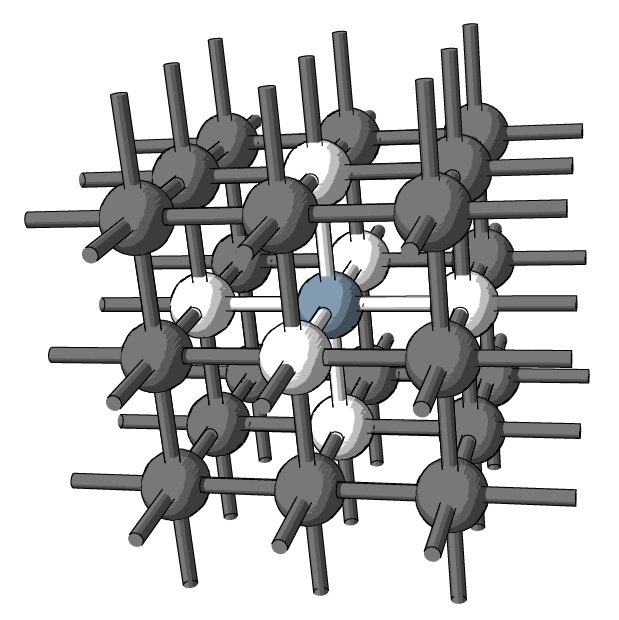
\includegraphics[width=0.48\columnwidth]{3dn6_lattice.png}
		\label{fig:lattice3dn6}
	}
	\caption{Common lattice structure for 2D and 3D image data. 
	\textbf{(a)} Simplest connection of neighbouring pixels for 2D images. Each non-edge pixel is connected to 4 pixels. This is 4-connectedness.
	\textbf{(b)} Simplest connection of neighbouring voxels for 3D images. Each non-edge voxel is connected to 6 voxles. This is 6-connectedness.}
	\label{fig:connectedness}
\end{figure}

\begin{figure}[!t]
	\centering
	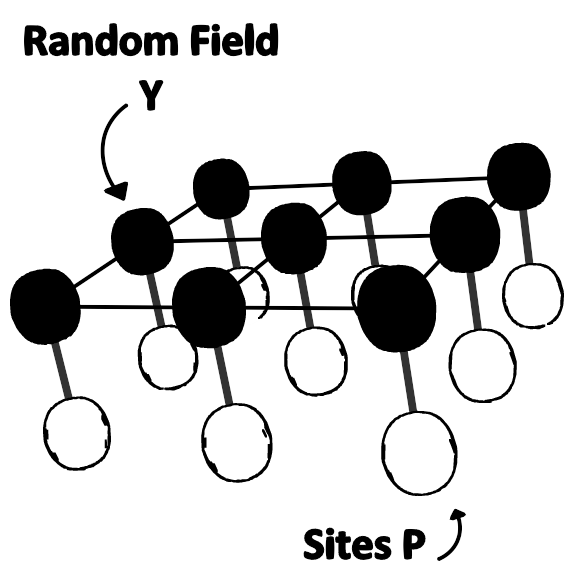
\includegraphics[width=0.35\columnwidth]{randomfield.png}
	\caption{4-connected random field $\mathbf{Y}$ over the sites $\mathcal{P}$.}
	\label{fig:randomfield}
\end{figure}

\begin{figure}[!t]
	\centering
	\subfigure[]
	{
		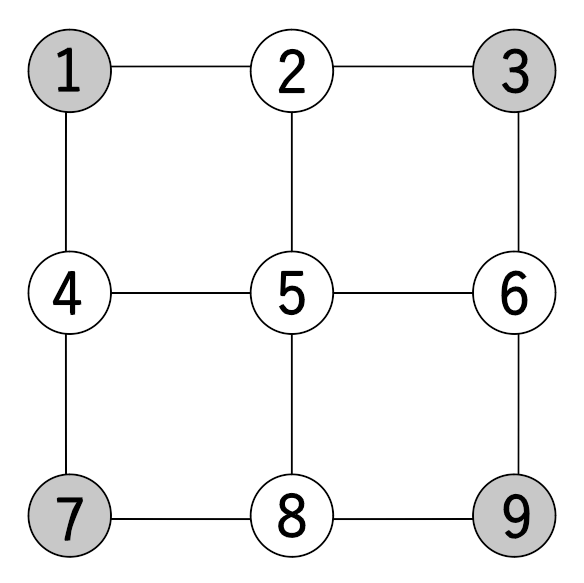
\includegraphics[width=0.35\columnwidth]{N4.png}
		\label{fig:n4}
	}
	\subfigure[]
	{
		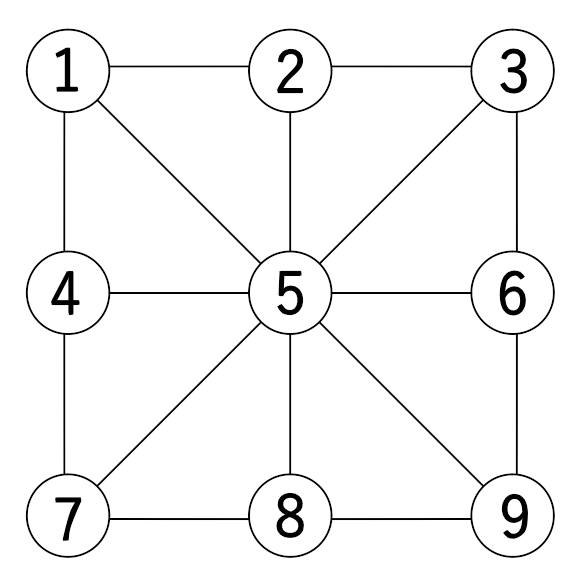
\includegraphics[width=0.35\columnwidth]{N8.png}
		\label{fig:n8}
	}
	\caption{Caption. \textbf{(a)} Caption. \textbf{(b)} Caption.}
	\label{fig:cliques}
\end{figure}

%----------------------------------------------------------------------------------------
%	SUBSECTION 2
%----------------------------------------------------------------------------------------

\subsection{MAP-MRF Estimation as Energy Minimisation}
\label{sec:MAPMRFEstimation}

The equivalence of MRFs and GRFs, proven by Hammersely-Clifford thereom, means that maximising \autoref{eq:mrfprobability} is equivalent to minimising \autoref{eq:gibbsenergy} \citep{Winkler2006}:

\begin{equation}
\mathbf{y^*} = \argmax_{\mathbf{y} \in \mathcal{Y}}\Pr(\mathbf{y}|\mathbf{x}) = \argmin_{\mathbf{y} \in \mathcal{Y}}E(\mathbf{y},\mathbf{x});
\label{eq:mrf_grf_equivaleance}
\end{equation}

the most probable labelling yields the lowest energy.
Obtaining the optimal labelling from \autoref{eq:mrf_grf_equivaleance} does not guarantee that the segmented output will be good.
The design of a good energy function, that captures all constraints and priors, is not easy.
However, optimisation is harder still.

From \autoref{eq:gibbs1}, if we take the negative log we get:

\begin{equation}
	-\log(\Pr(x|y)) = \log(Z) + \sum_{i \in \mathcal{V}}\Psi(x_i) + \sum_{(i,j) \in \mathcal{E}}\Psi_{i,j}(x_i,x_j),
\end{equation}

the constant $Z$ is not need as it does not affect the final labelling.
In this form, the equation is a sum of potentials, i.e. a sum of energies.
The first term encodes the data constraints, $E_{data}$, and the second term encodes the prior constraints, $E_{prior}$.
In addition, there is a factor that controls the relative importance between the data and the prior, $\lambda$.
The general form of the energy equation is:

\begin{equation}
	E(f) = E_{data}(f) + \lambda E_{prior}(f),
	\label{eq:generalform}
\end{equation}

where $f$ is a particular labelling.
The factor $\lambda$ encodes our belief in the prior i.e. the larger $\lambda$ is, the more we believe in the prior infomation.
The data energy takes on the following form:

\begin{equation}
	E_{data}(f) = \sum_{i \in \mathcal{V}} \Psi(x_i) =  \sum_{p \in \mathcal{P}}D_p(f_p).
	\label{eq:dataenergy}
\end{equation}

$D_p$ measures the level of agreement between the label $f_p$ and the pixel $p$.
A common approximation is to assume independency observations, and this makes designing $D_p$ relatively straightforward.
The only restriction is  $D_p(f_p) \in \Re^{+}$.
The prior energy takes on the following form:

\begin{equation}
	E_{prior}(f) = \sum_{(i,j) \in \mathcal{E}}\Psi_{i,j}(x_i,x_j) = \sum_{\{p,q\} \in \mathcal{N}}V_{\{p,q\}}(f_p,f_q).
	\label{eq:priorenergy}
\end{equation}

$V_{\{p,q\}}(f_p,f_q)$ is known as the \textit{neighbourhood interaction function}.
The aim of this function is to encourage neighbouring random variables to take on the same label, i.e. it penalises neighbouring pixels $p$ and $q$ if they have different labels.
The form of $V_{\{p,q\}}(f_p,f_q)$ is application dependant and is more tricky to design.
In image segmentation, the most common prior is that of smoothness, i.e intra-object pixel intensities are assumed to be the same or vary gradually within some range, it is at edges or boundaries where this assumption is violated.
The general form in \autoref{eq:generalform} can be rewritten as:

\begin{equation}
	E(f) = \sum_{p \in \mathcal{P}}D_p(f_p) + \lambda \sum_{\{p,q\} \in \mathcal{N}}V_{\{p,q\}}(f_p,f_q).
	\label{eq:generalformexpanded}
\end{equation}
 
 When we say MAP-MRF estimation we generally mean energy minimisation.
 Energy minimisation is a non-trivial task given the intractability of the search in the solution space.
 Energy minimisation can be catergorised into \textit{global energy minimisation} and \textit{local energy minimisation}.
 We briefly discuss some of the energy minimisation techniques.
 
\begin{definition}[Iterated Conditional Modes (ICM)]
	This is a deterministic method that converges to a local minimum \citep{Cassisa2010}.
	It a greedy technique that was introduced into vision by Besag \citep{Besag1986,Veksler1999}.
	The algorithm iteratively chooses the label that results in the largest decrease in energy at each site until convergence.
	It is extremely sensitive to initialisation as the dimensionality of the space increases with non-convex energies.
\end{definition}
 
\begin{definition}[Simulated Annealing]
	This is a stochastic optimisation method that simulates the annealing of a material.
	It is one of the only general-purpose energy minimisation methods.
	It was devloped and published independantly by \v{C}ern{\'y} \citep{Cerny1985} and Kirkpatrick \textit{et al.} \citep{Kirkpatrick1983} and was introduced into computer vision by Geman and Geman \citep{Geman1984}.
	The algorithm is initialised with a random labelling.
	Each pixel is then visited and a local random change is made.
	If the change results in a lower energy then it is accepted, else the change is accepted based on a probability parameter, i.e. the temperature.
	With certain cooling schedules the global minimum can be obtained however, this is horrendously slow in practise so sub-optimal schedules are used instead \citep{Geman1984}.
\end{definition}

\begin{definition}[Genetic Algorithms (GAs)]
 	GAs have been succesfully employed in energy minimisation for image segmentation \citep{MacEachern1998,Ballerini1999,Ballerini2001,Zeipelt2001,Ibanez2009}.
 	GAs work by performing simultaneous local searches that optimise the energy function via a random walk in the search space.
 	The algorithm terminates by choosing the search that found the lowest energy for the energy functional.
 	Their drawback is their inability to guarantee a global optimum \citep{McIntosh2013}.
\end{definition}

\begin{definition}[Gradient Descent]
	Explicit differentiation under the Euler-Lagrange equations can be used to obtain a solution \citep{McIntosh2013}.
	Each modified energy functional must be accompanied by derivation of obtaining a minimum \citep{Terzopoulos1987,Kass1988,Caselles1997,Chan2001}.
	With an artificial time step, this algorithm deforms a shape, using the gradient descent process, which is equated to the set of Euler-Lagrange equations.
	When the deformable models come to rest the equations are satisified.
	There are two common drawbacks with this method: Firstly, image noise can severely hinder the gradient descent process and this could lead to instability of the  deformation process.
	Secondly, increasing the number of dependant variables increases the complexity of the search space and time to converge to an optimal solution as there are more derivatives to calculate \citep{McIntosh2013}.
\end{definition}

\begin{definition}[Loopy Belief Propagation (LBP)]
	The belief propagation algorithm was initially designed to be used on acyclic graphs  where it able to obtain a global minimum \citep{Pearl1988}.
	However, the same algorithm has been succesfully applied on cyclic graphs firstly for error-correcting code problems \citep{Frey1998} and then later on in vision \citep{Freeman2000}.
	Convergence is not guaranteed as the algorithm might get stuck alternating between two labels \citep{Pearl1988}.
\end{definition}
  
\begin{definition}[Graph Cuts]
	Graph cuts have become an indespensable tool in computer vision.
	For a restrictive class of energy functions, \textit{submodular functions}, it is able to obtain a global minimum \citep{Kolmogorov2004,Boykov2001_2,Boykvo2001_3,Kolmogorov2007}.
	For non-submodular energy functions it is able to find approximate solutions with strong local optimality \citep{Boykov2001,Kohli2009,Komodakis2007,Kumar2009}.
	Greig \textit{et al.} was the first to use graph cuts in vision to find an exact solution to a certain energy function for the binary image restoration problem \citep{Greig1989}.
	However, it did recieve much attention and remained buried for almost ten years primarily because of the disinterest in binary image restoration and that, at the time, it's optimisation was notoriously slow which made it an unappealing technique when compared to stochastic optimisation methods, like simulated annealing, which was popular at the time.
	In the last two decades graph cut optimisation has been a major focus as a key tool in optimisation since Roy and Cox \citep{Roy1998} used it to solve more interesting problems in multi-camera stereo.
	Shortly after, Boykov \textit{et al.} generalised the method for determining the MAP estimate of MRFs \citep{Boykov1998}.
	Graph cut optimisation is the technique of focus in this thesis.
\end{definition}
  
%----------------------------------------------------------------------------------------
%	SECTION 3
%----------------------------------------------------------------------------------------

\section{Introduction to Graph Cuts}
\label{sec:GraphCuts}

Graph cuts is a combinatorial optimisation method which can be used to minimise energies of the form presented in \autoref{eq:generalformexpanded}. The aim of graph cuts is to partition a graph into mutual exclusive subgraphs by removing the edges whose sum of capacities is a minimum. We are interested with cutting the graph into two subgraphs. Graph cut algorithms existed long before their use was employed in vision, this is primarily due to the lack of computational power available at the time. Fortunately, computational power is no more as rare a resource as it was previously and this has paved a way into exploiting the power of graph data structures. As a result, this has also lead to vision-specific graph-cut algorithms. There are primarily three types of graph-cut algorithms: \textit{Augmenting Path Algorithms}, such as Ford-Fulkerson algorithm \citep{Ford1956}, Dinic algorithm \citep{Dinic1970}, Edmond-Karps algorithm \citep{Edmonds1972} etc, \textit{Preflow-Push Algorithms}, also known as \textit{Push-Relabel} \citep{Goldberg1988}, and \textit{Move-Making Algorithms} such as the $\alpha$-$\beta$ Swap \citep{Boykov2001}, $\alpha$-Expansion \citep{Boykov2001}, etc.

%----------------------------------------------------------------------------------------
%	SUBSECTION 1
%----------------------------------------------------------------------------------------

\subsection{Network Theory and the Min-cut Problem}
\label{sec:NetworkTheory}

In this section we briefly cover the foundation aspects to understanding graph cuts. We cover \textit{Flow networks}, a branch of Graph Theory also known as \textit{Transportation networks}, and introduce the \textit{Min-cut problem}. For a solid understanding in Graph Theory and Flow Networks see \citep{Deo1974,Bondy1976,Steen2010,Newman2010}. A brief introduction is given in \Cref{AppendixB}.

\begin{definition}[Network]
	A network $\textbf{N} = (V,E)$ is a directed graph with a source node $s$, a sink node $t$ and a strictly positive capacity on every edge. That is, for each edge $e \in E$, the capacity, $c(.)$, obeys $c(e) \in \Re^{+}$.
	The \textbf{source node} only has out-going edges, $d_{in}(s) = 0$ and $d_{out}(s) \geq 0$. The \textbf{sink node} only has incoming edges, $d_{in} \geq 0$ and $d_{out} = 0$. An example of a network is illustrated in \Cref{fig:network}.
\end{definition}

\tikzstyle{vertex}=[circle,thick,draw]
\tikzstyle{edge} = [draw=black!24, very thick,->]
\tikzstyle{weight} = [font=\small]
\begin{figure}[!h]
	\centering
	\resizebox {\columnwidth} {!} {
%		[scale=1.5, auto, swap, background rectangle/.style={fill=blue!10}, show background rectangle, >={Stealth[black!24]}]
		\begin{tikzpicture}[scale=1.5, auto, swap, background rectangle/.style={fill=blue!10}, >={Stealth[black!24]}]
		\draw[black] node at (-0.2,1.5) [font=\large,right,rounded corners,inner sep=1ex] {$\textbf{N}$};
		
		\draw node[circle,thick,right,fill=red!20,text=red!20] at (-0.2,0) {$s$};
		\draw node[circle,thick,right,fill=red!20,text=red!20] at (5.8,0) {$t$};
		\draw[dashed,draw=red!24,very thick] (0.0,0) -- (0.5,-1.5);
		\draw[dashed,draw=red!24,very thick] (6.0,0) -- (6.5,-1.5);
		\draw[dashed,draw=red!24,very thick] (2.65,1.25) -- (4,1.5);
		
		% draw the vertices
		\foreach \pos/\name in {{(0,0)/s},{(2,1)/a},{(4,1)/b},{(2,-1)/c},{(4,-1)/d}, {(6,0)/t}}
		\node[vertex] (\name) at \pos {$\name$};
		% connect vertices with edges and draw weights
		\foreach \source/ \dest /\weight in {s/a/7,s/c/2,a/b/{},c/d/2,b/t/5,d/t/3}
		\path[edge] (\source) edge node[weight] {$\weight$} (\dest);
		% bends
		\path [draw=black!24, very thick,->] (a) edge[bend left=-30] node {$3$} (d);
		\path [draw=black!24, very thick,->] (c) edge[bend left=30] node {$3$} (b);
		% info box		
		\draw node[circle,right,fill=red!20] at (2.65,1.25) {$5$};
		\draw node[right,rounded corners,fill=red!20,inner sep=1ex] at (4,1.5){$capacity$};
		\draw node[right,rounded corners,fill=red!20,inner sep=1ex] at (0,-1.5){$source$};
		\draw node[right,rounded corners,fill=red!20,inner sep=1ex] at (6,-1.5){$sink$};
		% s	
		\draw[orange] node at (-0.2,0.4) [font=\footnotesize,right,rounded corners,inner sep=1ex] {$d_{in}=0$};
		\draw[orange] node at (-0.2,0.7) [font=\footnotesize,right,rounded corners,inner sep=1ex] {$d_{out}=2$};	
		% t
		\draw[orange] node at (5.8,0.4) [font=\footnotesize,right,rounded corners,inner sep=1ex] {$d_{in}=2$};
		\draw[orange] node at (5.8,0.7) [font=\footnotesize,right,rounded corners,inner sep=1ex] {$d_{out}=0$};
		\end{tikzpicture}
	}
	\caption{Network \textbf{N} with no flow. The in-degree and out-degree for the source, \textbf{s}, and the sink, \textbf{t}, are shown next to the corresponding node.}
	\label{fig:network}
\end{figure}

\begin{definition}[Flow]
	A flow $f : V^2 \longrightarrow \Re^{+}$ is associated with each edge $e = (u,v)$ such that:
	\begin{enumerate}
		\item for each edge $e \in E$ we have $0 \leq f(e) \leq c(e)$. That is, the flow is positive and cannot excees the capacity of the edge.
		
		\item for each intermediate node $v \in V\setminus \{s,t\}$ the in- and out-flow of that node $\sum_{u \in V^-(v)} f(u,v) = \sum_{u \in V^+(v)} f(v,u)$.
	\end{enumerate}
	The \textbf{total flow} $F$ of a network is then what leaves the source $s$ or reaches the sink $t$:
	\begin{equation}
	F(\textbf{N}) := \sum_{u \in V} f(s,u) - \sum_{u \in V}f(u,s) = \sum_{u \in V} f(u,t) - \sum_{u \in V}f(t,u)
	\end{equation}
	An example of a network with non-zero flow is illustrated in \Cref{fig:networkwithflow}.
\end{definition}

\tikzstyle{vertex}=[circle,thick,draw]
\tikzstyle{edge} = [draw=black!24, very thick,->]
\tikzstyle{weight} = [font=\small]
\begin{figure}[!h]
	\centering
	\resizebox {\columnwidth} {!} {
%		[scale=1.5, auto, swap, background rectangle/.style={fill=blue!10}, show background rectangle, >={Stealth[black!24]}]
		\begin{tikzpicture}[scale=1.5, auto, swap, background rectangle/.style={fill=blue!10}, >={Stealth[black!24]}]
		\draw[black] node at (-0.2,1.5) [font=\large,right,rounded corners,inner sep=1ex] {$\textbf{N}$};
		\draw node[circle,thick,right,fill=red!20,text=red!20] at (-0.2,0) {$s$};
		\draw node[circle,thick,right,fill=red!20,text=red!20] at (5.8,0) {$t$};
		\draw[dashed,draw=red!24,very thick] (2.65,1.25) -- (4,1.5);
		\draw[dashed,draw=red!24,very thick] (0.0,0) -- (0.5,-1.5);
		\draw[dashed,draw=red!24,very thick] (6.0,0) -- (5.5,-1.5);
		% draw the vertices
		\foreach \pos/\name in {{(0,0)/s},{(2,1)/a},{(4,1)/b},{(2,-1)/c},{(4,-1)/d}, {(6,0)/t}}
		\node[vertex] (\name) at \pos {$\name$};
		% connect vertices with edges and draw weights
		\foreach \source/ \dest /\weight in {s/a/{7/5},s/c/{2/2},a/b/{},c/d/{2/1},b/t/{5/4},d/t/{3/3}}
		\path[edge] (\source) edge node[weight] {$\weight$} (\dest);
		% bends
		\path [draw=black!24, very thick,->] (a) edge[bend left=-30] node {$3/1$} (d);
		\path [draw=black!24, very thick,->] (c) edge[bend left=30] node {$3/2$} (b);
		% info box		
		\draw node[rounded corners,right,fill=red!20] at (2.65,1.25) {$5/3$};
		\draw node[right,rounded corners,fill=red!20,inner sep=1ex] at (4,1.5){$capacity/flow$};
		% s	
		\draw node[right,rounded corners,fill=red!20,inner sep=1ex] at (0,-1.5) [font=\footnotesize,right,rounded corners,inner sep=1ex] {$\sum\limits_{u \in V_N} f(s,u)=7$};
		% t
		\draw node[right,rounded corners,fill=red!20,inner sep=1ex] at (4.6,-1.5) [font=\footnotesize,right,rounded corners,inner sep=1ex] {$\sum\limits_{u \in V_N} f(u,t)=7$};
		\end{tikzpicture}
	}
	\caption{Network \textbf{N} with flow. The flow out of the source node, \textbf{s}, is equal to the flow into the sink node, \textbf{t}. For all other nodes, the flow-in is equal to the flow-out. This is the conservation of flow principle. This is only part of the network. The remaining part is the residual graph which shows the amount of reverse flow is available on an edge.}
	\label{fig:networkwithflow}
\end{figure}

\begin{definition}[Cut]
	A cut of a network $\textbf{N} = (V,E)$ is a partitioning of the vertex set $V = P \bigcup \bar{P}$ into two disjoint sets $P$ containining the source node $s$ and $\bar{P}$ containing the sink node $t$. $P \bigcap \bar{P} = \emptyset$.
	The \textbf{cost} of a cut is the sum of the capacity of the edges $(u,v) \in V$ where $u \in P$ and $v \in \bar{P}$:
	\begin{equation}
	\kappa (P, \bar{P}) = \sum_{u \in P; v \in \bar{P}} c(u,v)
	\end{equation}
	A network with a valid cut is illustrated in \Cref{fig:validcut}. Invalid cuts are shown for the same network in \Cref{fig:invalidcut1} and \Cref{fig:invalidcut2}.
\end{definition}

\tikzstyle{vertex}=[circle,thick,draw]
\tikzstyle{edge} = [draw=black!24, very thick,->]
\tikzstyle{weight} = [font=\small]
\begin{figure}[!h]
	\centering
	\resizebox {\columnwidth} {!} {
%		[scale=1.5, auto, swap, background rectangle/.style={fill=blue!10}, show background rectangle, >={Stealth[black!24]}]
		\begin{tikzpicture}[scale=1.5, auto, swap, background rectangle/.style={fill=blue!10}, >={Stealth[black!24]}]
		\draw[black] node at (-0.2,1.5) [font=\large,right,rounded corners,inner sep=1ex] {$\textbf{N}$};
		\path[fill=red!20,,use Hobby shortcut,closed=true] (-0.3,-0.1) .. (1,1) .. (2.3,1.2) .. (1.3,0.2);
		%		\draw node[text=blue] at (-0.3,0) {$1$};
		%		\draw node[text=blue] at (1,1) {$2$};
		%		\draw node[text=blue] at (2.5,1.2) {$3$};
		%		\draw node[text=blue] at (1,0.0) {$4$};
		\path[fill=blue!20,,use Hobby shortcut,closed=true] (1.5,-1) .. (2.5,0.5) .. (3.5,1.2) .. (5.2,1.0) .. (6.3,0.0) .. (5.0,-1);
		%		\draw node[text=blue] at (1,-1) {$1$};
		%		\draw node[text=blue] at (3.2,1.2) {$2$};
		%		\draw node[text=blue] at (5.0,1.2) {$3$};
		%		\draw node[text=blue] at (6.5,0.0) {$4$};
		% draw the vertices
		\foreach \pos/\name in {{(0,0)/s},{(2,1)/a},{(4,1)/b},{(2,-1)/c},{(4,-1)/d}, {(6,0)/t}}
		\node[vertex] (\name) at \pos {$\name$};
		% connect vertices with edges and draw weights
		\foreach \source/ \dest /\weight in {s/a/{},s/c/{},a/b/{},c/d/{},b/t/{},d/t/{}}
		{
			\path[edge] (\source) edge node[weight] {$\weight$} (\dest);
		}		
		% bends
		\path [draw=black!24,very thick,->,name path=curve1] (a) edge[bend left=-30] node {} (d);
		\path [draw=black!24,very thick,->,name path=curve2] (c) edge[bend left=30] node {} (b);
		% cut
		\draw node [text=orange] at (0,-0.7) {$C$};
		\path[dashed, very thick, draw=orange, name path=C] (0,-1) -- (3.5,1.5);
		% intersections
		\path [draw=black!24,name path=line1] (s) -- (c);		
		\path [draw=black!24,name path=line2] (a) -- (b);		
		\path [draw=blue!24,name path=line3] (a) edge [bend left=-30] (d);
		\fill [color=orange, name intersections={of=C and line1}] (intersection-1) circle (2pt);
		\fill [color=orange, name intersections={of=C and line2}] (intersection-1) circle (2pt);
		\fill [color=orange, name intersections={of=C and line3}] (2.15,0.53) circle (2pt);	
		% info box
		\draw[yshift=-2.1cm,xshift=-0.5cm]
		node [right,rounded corners,fill=orange!20,inner sep=1ex]
		{
			$S = \{s,a\}$, \, $T = \{t,b,c,d\}$, \,$C = \{(sc), (ab), (ad)\}$
		};
		\end{tikzpicture}
	}
	\caption{Network \textbf{N} with with a valid cut \textbf{C}. The nodes within the red region are reachable from the source and the nodes within the blue region are able to reach the sink. The cut set, \textbf{C}, is show in the orange filled block.}
	\label{fig:validcut}
\end{figure}

\tikzstyle{vertex}=[circle,thick,draw]
\tikzstyle{edge} = [draw=black!24, very thick,->]
\tikzstyle{weight} = [font=\small]
\begin{figure}[!h]
	\centering
	\resizebox {\columnwidth} {!} {
%		[scale=1.5, auto, swap, background rectangle/.style={fill=blue!10}, show background rectangle, >={Stealth[black!24]}]
		\begin{tikzpicture}[scale=1.5, auto, swap, background rectangle/.style={fill=blue!10}, >={Stealth[black!24]}]
		\draw[black] node at (-0.2,1.5) [font=\large,right,rounded corners,inner sep=1ex] {$\textbf{N}$};
		\path[fill=red!20,,use Hobby shortcut,closed=true] (-0.3,-0.1) .. (2,1.5) .. (4,1.5) .. (6.4,-0.1) .. (4,0) .. (2,0) ;
		%				\draw node[text=blue] at (-0.3,0) {$1$};
		%				\draw node[text=blue] at (2,1.5) {$2$};
		%				\draw node[text=blue] at (4,1.5) {$3$};
		%				\draw node[text=blue] at (6.3,0.0) {$4$};
		%				\draw node[text=blue] at (4,0.0) {$5$};
		%				\draw node[text=blue] at (2,0.0) {$6$};
		\path[fill=blue!20,,use Hobby shortcut,closed=true] (1.5,-1) .. (3.0,-0.7) .. (4.5,-1.0) .. (3.0,-1.2);
		%				\draw node[text=blue] at (1.5,-1) {$1$};
		%				\draw node[text=blue] at (3.0,-0.7) {$2$};
		%				\draw node[text=blue] at (4.5,-1.0) {$3$};
		%				\draw node[text=blue] at (3.0,-1.2) {$4$};			
		% draw the vertices
		\foreach \pos/\name in {{(0,0)/s},{(2,1)/a},{(4,1)/b},{(2,-1)/c},{(4,-1)/d}, {(6,0)/t}}
		\node[vertex] (\name) at \pos {$\name$};
		% connect vertices with edges and draw weights
		\foreach \source/ \dest /\weight in {s/a/{},s/c/{},a/b/{},c/d/{},b/t/{},d/t/{}}
		{
			\path[edge] (\source) edge node[weight] {$\weight$} (\dest);
		}		
		% bends
		\path [draw=black!24,very thick,->,name path=curve1] (a) edge[bend left=-30] node {} (d);
		\path [draw=black!24,very thick,->,name path=curve2] (c) edge[bend left=30] node {} (b);
		% cut
		\draw node [text=orange] at (0,-0.7) {$C$};
		\path[dashed, very thick, draw=orange, name path=C] (0,-1) edge[bend left=30] (6,-1);
		% intersections
		\fill [color=orange] (1.0,-0.5) circle (2pt);
		\fill [color=orange] (5.0,-0.5) circle (2pt);
		\fill [color=orange] (2.28,-0.18) circle (2pt);
		\fill [color=orange] (2.52,-0.165) circle (2pt);
		% info box
		%		\draw[yshift=-2.1cm,xshift=-0.5cm]
		%		node [right,rounded corners,fill=orange!20,inner sep=1ex]
		%		{
		%			$S = \{s,a\}$, \, $T = \{t,b,c,d\}$, \,$C = \{(sc), (ab), (ad)\}$
		%		};
		\end{tikzpicture}
	}
	\caption{Network \textbf{N} with with a invalid cut \textbf{C}. The cut does not partition source node \textbf{s} and sink node \textbf{t} into distinct sets.}
	\label{fig:invalidcut1}
\end{figure}

\tikzstyle{vertex}=[circle,thick,draw]
\tikzstyle{edge} = [draw=black!24, very thick,->]
\tikzstyle{weight} = [font=\small]
\begin{figure}[!h]
	\centering
	\resizebox {\columnwidth} {!} {
%		[scale=1.5, auto, swap, background rectangle/.style={fill=blue!10}, show background rectangle, >={Stealth[black!24]}]
		\begin{tikzpicture}[scale=1.5, auto, swap, background rectangle/.style={fill=blue!10}, >={Stealth[black!24]}]
		\draw[black] node at (-0.2,1.5) [font=\large,right,rounded corners,inner sep=1ex] {$\textbf{N}$};
		%		\path[fill=red!20,,use Hobby shortcut,closed=true] (-0.3,-0.1) .. (2,1.5) .. (4,1.5) .. (6.4,-0.1) .. (4,0) .. (2,0) ;
		%				\draw node[text=blue] at (-0.3,0) {$1$};
		%				\draw node[text=blue] at (2,1.5) {$2$};
		%				\draw node[text=blue] at (4,1.5) {$3$};
		%				\draw node[text=blue] at (6.3,0.0) {$4$};
		%				\draw node[text=blue] at (4,0.0) {$5$};
		%				\draw node[text=blue] at (2,0.0) {$6$};
		%		\path[fill=blue!20,,use Hobby shortcut,closed=true] (1.5,-1) .. (3.0,-0.7) .. (4.5,-1.0) .. (3.0,-1.2);
		%				\draw node[text=blue] at (1.5,-1) {$1$};
		%				\draw node[text=blue] at (3.0,-0.7) {$2$};
		%				\draw node[text=blue] at (4.5,-1.0) {$3$};
		%				\draw node[text=blue] at (3.0,-1.2) {$4$};			
		% draw the vertices
		\foreach \pos/\name in {{(0,0)/s},{(2,1)/a},{(4,1)/b},{(2,-1)/c},{(4,-1)/d}, {(6,0)/t}}
		\node[vertex] (\name) at \pos {$\name$};
		% connect vertices with edges and draw weights
		\foreach \source/ \dest /\weight in {s/a/{},s/c/{},a/b/{},c/d/{},b/t/{},d/t/{}}
		{
			\path[edge] (\source) edge node[weight] {$\weight$} (\dest);
		}		
		% bends
		\path [draw=black!24,very thick,->,name path=curve1] (a) edge[bend left=-30] node {} (d);
		\path [draw=black!24,very thick,->,name path=curve2] (c) edge[bend left=30] node {} (b);
		% cut
		\draw node [text=orange] at (0,-0.7) {$C$};
		\draw [dashed, orange, very thick] plot [smooth] coordinates {(0,-1) (2.5,1) (3,1.2) (3.5,-1.5)};
		% intersections
		\fill [color=orange] (0.77,-0.37) circle (2pt);
		\fill [color=orange] (2.09,0.68) circle (2pt);
		\fill [color=orange] (2.5,1) circle (2pt);
		\fill [color=orange] (3.05,1) circle (2pt);
		\fill [color=orange] (3.12,0.7) circle (2pt);
		\fill [color=orange] (3.40,-0.82) circle (2pt);
		\fill [color=orange] (3.42,-1) circle (2pt);
		% info box
		%		\draw[yshift=-2.1cm,xshift=-0.5cm]
		%		node [right,rounded corners,fill=orange!20,inner sep=1ex]
		%		{
		%			$S = \{s,a\}$, \, $T = \{t,b,c,d\}$, \,$C = \{(sc), (ab), (ad)\}$
		%		};
		\end{tikzpicture}
	}
	\caption{Network \textbf{N} with with a invalid cut \textbf{C}. The cut partition partitions the graph into more than two sets and the cut intersects the edges $ab$ and $ad$ twice.}
	\label{fig:invalidcut2}
\end{figure}

\begin{definition}[Maximal Flow]
	The largest amount of flow that is able to reach the sink from the source is known as the maximal flow.  A network with a maximal flow, also known as a \textit{max-flow}, is illustrated in \Cref{fig:maxflow}.
\end{definition}

\tikzstyle{vertex}=[circle,thick,draw]
\tikzstyle{edge} = [draw=black!24, very thick,->]
\tikzstyle{weight} = [font=\small]
\begin{figure}[!h]
	\centering
	\resizebox {\columnwidth} {!} {
%		[scale=1.5, auto, swap, background rectangle/.style={fill=blue!10}, show background rectangle, >={Stealth[black!24]}]
		\begin{tikzpicture}[scale=1.5, auto, swap, background rectangle/.style={fill=blue!10}, >={Stealth[black!24]}]
		\draw[black] node at (-0.2,1.5) [font=\large,right,rounded corners,inner sep=1ex] {$\textbf{N}$};
		\draw node[circle,thick,right,fill=red!20,text=red!20] at (-0.2,0) {$s$};
		\draw node[circle,thick,right,fill=red!20,text=red!20] at (5.8,0) {$t$};
		\draw[dashed,draw=red!24,very thick] (0.0,0) -- (0.5,-1.5);
		\draw[dashed,draw=red!24,very thick] (6.0,0) -- (5.5,-1.5);
		% draw the vertices
		\foreach \pos/\name in {{(0,0)/s},{(2,1)/a},{(4,1)/b},{(2,-1)/c},{(4,-1)/d}, {(6,0)/t}}
		\node[vertex] (\name) at \pos {$\name$};
		% connect vertices with edges and draw weights
		\foreach \source/ \dest /\weight in {s/a/{7/6},s/c/{2/2},a/b/{5/5},c/d/{2/2},b/t/{5/5},d/t/{3/3}}
		\path[edge] (\source) edge node[weight] {$\weight$} (\dest);
		% bends
		\path [draw=black!24, very thick,->] (a) edge[bend left=-30] node {$3/0$} (d);
		\path [draw=black!24, very thick,->] (c) edge[bend left=30] node {$3/1$} (b);
		%info
		% s	
		\draw node[right,rounded corners,fill=red!20,inner sep=1ex] at (0,-1.5) [font=\footnotesize,right,rounded corners,inner sep=1ex] {$\sum\limits_{u \in V_N} f(s,u)=8$};
		% t
		\draw node[right,rounded corners,fill=red!20,inner sep=1ex] at (4.6,-1.5) [font=\footnotesize,right,rounded corners,inner sep=1ex] {$\sum\limits_{u \in V_N} f(u,t)=8$};
		\end{tikzpicture}
	}
	\caption{Network \textbf{N} with maximum flow. There is no way to push more flow out of the source into the sink without breaking the rules for the conservation of flow.}
	\label{fig:maxflow}
\end{figure}

\begin{definition}[Minimal Cut]
	A cut $C$ on a network $\textbf{N} = (V,E)$ is a minimal cut if there exists no other cut $C'$ where $\kappa (C') < \kappa(C)$. A network with a minimal cut, also known as a \textit{min-cut}, is illustrated in \Cref{fig:mincut}.
\end{definition}

\tikzstyle{vertex}=[circle,thick,draw]
\tikzstyle{edge} = [draw=black!24,very thick,->]
\tikzstyle{weight} = [font=\small]
\begin{figure}[!h]
	\centering
	\resizebox {\columnwidth} {!} {
%		[scale=1.5, auto, swap, background rectangle/.style={fill=blue!10}, show background rectangle, >={Stealth[black!24]}]
		\begin{tikzpicture}[scale=1.5, auto, swap, background rectangle/.style={fill=blue!10}, >={Stealth[black!24]}]
		\draw[black] node at (-0.2,1.5) [font=\large,right,rounded corners,inner sep=1ex] {$\textbf{N}$};	
		\path[fill=red!20,,use Hobby shortcut,closed=true] (-0.3,-0.1) .. (2,1.5) .. (4,1.5) .. (4.5,-0.1) .. (4,-1.5) .. (2,-1.5) ;
		%			\draw node[text=blue] at (-0.3,0) {$1$};
		%			\draw node[text=blue] at (2,1.5) {$2$};
		%			\draw node[text=blue] at (4,1.5) {$3$};
		%			\draw node[text=blue] at (6.3,0.0) {$4$};
		%			\draw node[text=blue] at (4,-1.5) {$5$};
		%			\draw node[text=blue] at (2,-1.5) {$6$};
		\path[fill=blue!20,use Hobby shortcut,closed=true] (5.5,0) .. (6.0,0.5) .. (6.5,0) .. (6.0,-0.5);
		%			\draw node[text=blue] at (5.5,0) {$1$};
		%			\draw node[text=blue] at (6.0,0.5) {$2$};
		%			\draw node[text=blue] at (6.5,0) {$3$};
		%			\draw node[text=blue] at (6.0,-0.5) {$4$};
		% draw the vertices
		\foreach \pos/\name in {{(0,0)/s},{(2,1)/a},{(4,1)/b},{(2,-1)/c},{(4,-1)/d}, {(6,0)/t}}
		\node[vertex] (\name) at \pos {$\name$};
		% connect vertices with edges and draw weights
		\foreach \source/ \dest /\weight in {s/a/7,s/c/2,a/b/{5},c/d/2,b/t/5,d/t/3}
		\path[edge] (\source) edge node[weight] {$\weight$} (\dest);
		% bends
		\path [draw=black!24, very thick,->] (a) edge[bend left=-30] node {$3$} (d);
		\path [draw=black!24, very thick,->] (c) edge[bend left=30] node {$3$} (b);
		% cut
		\draw node [text=orange] at (4.8,-1.0) {$C$};
		\path[dashed, very thick, draw=orange, name path=C] (5,-1.2) -- (5,1.2);
		% intersections
		\path [draw=black!24,name path=line1] (b) -- (t);
		\path [draw=black!24,name path=line2] (d) -- (t);
		\fill [color=orange, name intersections={of=C and line1}] (intersection-1) circle (2pt);
		\fill [color=orange, name intersections={of=C and line2}] (intersection-1) circle (2pt);
		%info
		% minimum capacity	
		\draw node[right,rounded corners,fill=orange!20,inner sep=1ex] at (5,-1.5) [font=\footnotesize,right,rounded corners,inner sep=1ex] {$\sum\limits_{e \in C} c(e)=8$};
		\end{tikzpicture}
	}
	\caption{Network \textbf{N} with minimal cut \textbf{C}. The sum of the capacity of all the edges in the cut set is the minimum of all possible valid cuts on the network \textbf{N}.}
	\label{fig:mincut}
\end{figure}

\textcolor{red}{Talk about the max-flow/min-cut duality, non-uniqueness.}
%In the next section we show that the Maximal Flow problem and the Minimal Cut problem are duals of each other, commonly known as the Max-Flow/Min-Cut problem.
In \Cref{fig:maxflow} and \Cref{fig:mincut} the maximum flow and the minimum cut yield the same answer. This is not a coincidence, in fact the two problems are duals of each other, known as the \textit{max-flow min-cut duality}. This was proven by P. Elias, A. Feinstein, and C.E. Shannon \citep{Elias1956} and by Ford and Fulkerson \citep{Ford1956} independently in 1956. This duality is immensely helpful in developing machine algorithms to compute the minimum, since it is easier to find a maximum flow. It is important to realise that there maybe many cuts that can be minimum cut and many flow configurations that can yield the maximum flow, hence the solution is not guaranteed to be unique only an optimum.

%----------------------------------------------------------------------------------------
%	SUBSECTION 2
%----------------------------------------------------------------------------------------

\subsection{Image Segmentation Graph Structure}
\label{sec:GraphCutFramework}

\textcolor{red}{Graph construction. Special terminology: n-links, t-links, etc. Undirected to directed conversion. Labels as terminals. Construction with and withtout seeds. Edge weighting -> leave submodular functions to their own section.}
In graph cut image segmentation the energy function, defined by the image, has to be represented as a graph, specifically a network. We now look at how to 2D binary segmentation energy is constructed as a graph. The graph that is constructed uses the MRF, \Cref{sec:MarkovRandomFields}, model of the image as its base. Each pixel is a node in the graph. The connections between "pixel nodes" are bi-directional, which is generally decomposed into two uni-directional edges, and are known as \textit{n-links} which is synonymous with \textit{neighbour-links}. Additionally, each label is also represented as a node. Each "pixel node" is attached to all "label nodes". In binary, segmentation, there are two labels i.e. object and background. The edges that connect "label nodes" to "pixel nodes" are called \textit{t-links} which is synonymous with \textit{terminal-links}. In keeping with network construction, one label will be the source and the other will be the sink. The t-link weights are generally learned from user input seeds or automatically generated seeds. Seeds mark which type of pixels belong to the object and which belong to the background, an illustration is shown in \Cref{fig:graph_image}. With the seed data and the neighbourhood interaction, we can construct a graph representation of the energy to be minimised over the image as illustrated in \Cref{fig:graph_graph}. Once a graph has been constructed, we then call upon a max-flow/min-cut method which will minimise the energy function by partitioning the graph into two subgraphs, as shown in \Cref{fig:graph_graphcut}. All pixels are classified according to which "label node" they're still attached to after the max-flow/min-cut algorithm has run, this is illustrated in \Cref{fig:graph_mask}.

\begin{figure}[!t]
	\centering
	\subfigure[]
	{
		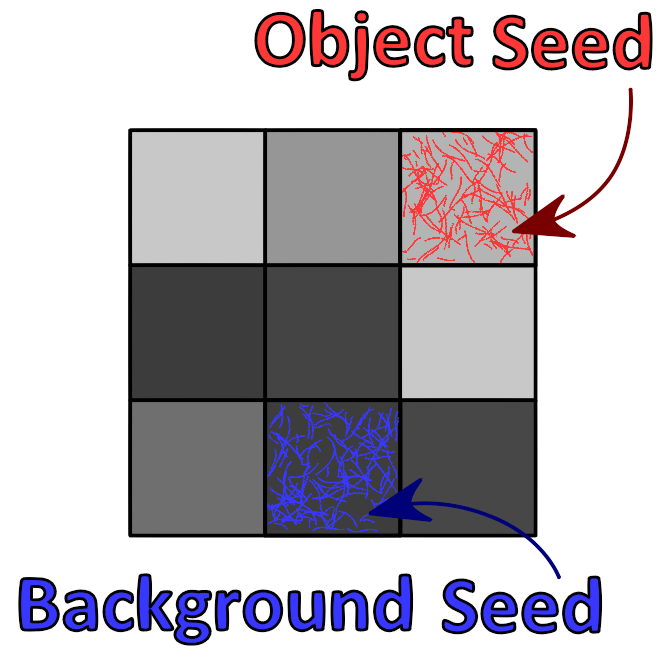
\includegraphics[width=0.45\columnwidth]{graph_construction_image.png}
		\label{fig:graph_image}
	}
	\subfigure[]
	{
		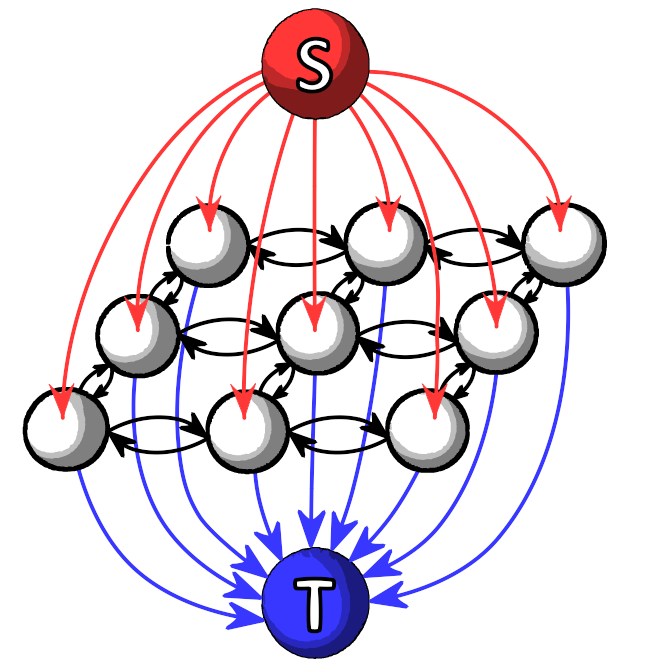
\includegraphics[width=0.45\columnwidth]{graph_construction_graph.png}
		\label{fig:graph_graph}
	}
	\subfigure[]
	{
		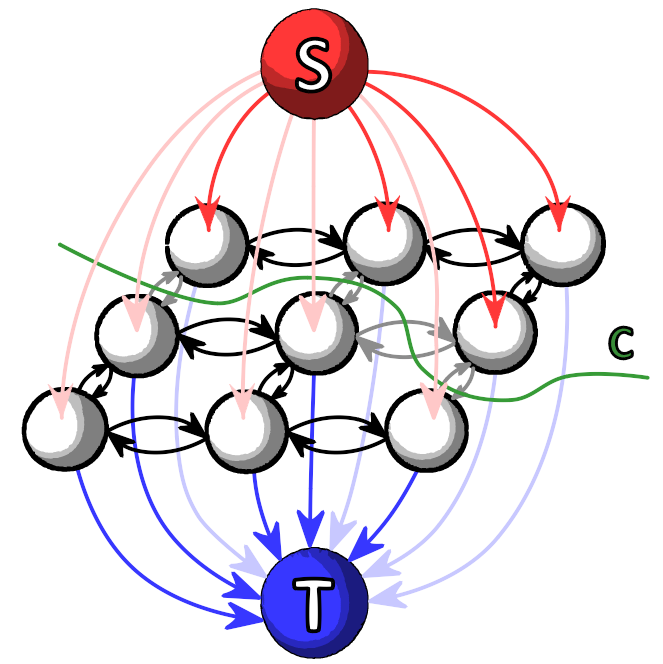
\includegraphics[width=0.45\columnwidth]{graph_construction_graphcut.png}
		\label{fig:graph_graphcut}
	}
	\subfigure[]
	{
		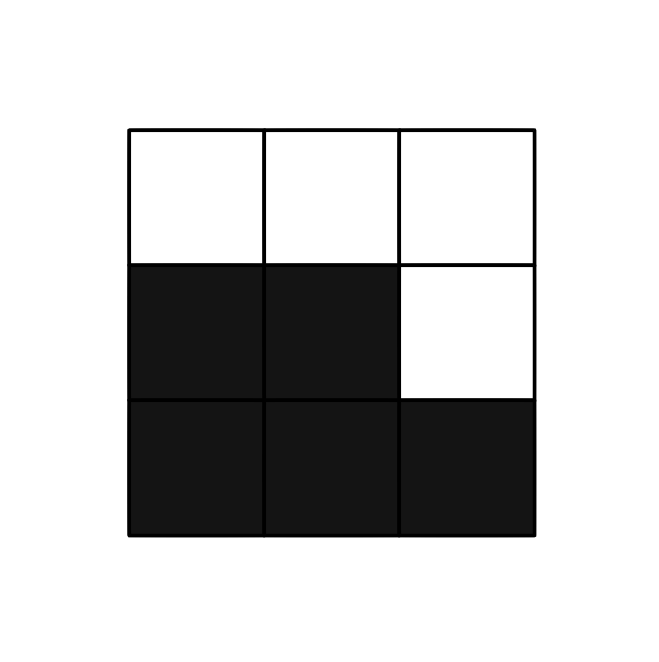
\includegraphics[width=0.45\columnwidth]{graph_construction_mask.png}
		\label{fig:graph_mask}
	}
	\caption{Overall process of the graph cut image segmentation process.
	\textbf{(a)} Image with object and background seeds.
	\textbf{(b)} Graph representation of the energy function to be minimised over the image. The n-links are represented by black arrows, the t-links from the source are shown in red, and the t-links to the sink are shown in blue.
	\textbf{(c)} Minimised energy function by cut C. The light red, light blue and grey edges are those that belong to the cut set C.
	\textbf{(d)} Segmentation mask after label assignment. In this case, all nodes that are still attached to the source, their corresponding pixel label is shown in white, similarly, nodes that are connected to the sink have their corresponding pixel labels shown in black.}
	\label{fig:graphcut_process}
\end{figure}

%----------------------------------------------------------------------------------------
%	SUBSECTION 3
%----------------------------------------------------------------------------------------

\subsection{Submodular Functions}
\label{sec:SubmodularFunctions}

In the previous section we talked about representing the energy function as a graph. However, not all energy functions can be represented as a graph. Moreover, minimising an arbitrary energy function, even if the energy is binary, is NP-hard \citep{Shimony1994}. There does exist a class of functions which is graph representable and is able to be minimised in polynomial time, i.e. an exact global minimum can be obtained in a single graph cut. These energy functions are known as \textit{submodular functions}. They are sometimes referred to as "discrete analog of convex functions" since they're the easiest to minimise, much like convex functions. For an energy to be submodular, it must satisfy the submodularity constraint:

\begin{align}
&f^p(a,b) + f^p(a+1,b+1) \leq f^p(a,b+l) + f^p(a+1,b),&  &\forall a,b \in \mathcal{L},&
\end{align}

where $\mathcal{L}$ is an ordered label set. The type of energies we are concerned with are second order binary energies, and enforcing the submodularity constraint means that the energy function must to satisfy:

\begin{align}
&E_{ij}(0,0) + E_{ij}(1,1) \leq E_{ij}(0,1) + E_{ij}(1,0),&  &\forall \{i,j\} \in \mathcal{N},&
\label{eq:submodular_energy}
\end{align}

where $\mathcal{L}=\{0,1\}$. It is necessary and sufficient for an energy function to satisfy \Cref{eq:submodular_energy} to compute the exact global minimum in polynomial time in a single graph cut. This was first characterised by Kolomogorov and Zabih \citep{Kolmogorov2004}.

%----------------------------------------------------------------------------------------
%	SECTION 4
%----------------------------------------------------------------------------------------

\section{Graph Cut Algorithms for Energy Minimisation}
\label{sec:MaxFlowMinCutAlgoithms}

Image segmentation via graph cuts can be seen as three main stages. Firstly the problem is modelled and a suitable energy function is designed. Generally, this is a trade-off between accuracy and constraining to the submodularity constraint. Secondly, a graph is constructed which represents the energy function. Thirdly, and finally, the energy function is minimised by using a max-flow/min-cut algorithm. In this section we discuss the last stage. The minimisation algorithms are either general or specific to the energy functions. We briefly discuss some of the most common max-flow algorithms.

%-----------------------------------
%	SUBSECTION 1
%-----------------------------------
\subsection{Ford-Fulkerson}
\label{sec:FordFulkerson}

The Ford-Fulkerson max-flow algorithm \citep{Ford1956} is designed to on an arbitrary network with one source and one sink. Ford and Fulkerson proved that the max-flow and min-cut problems are duals of each other, hence solving one means that you've obtained the solution to the other. Augmenting path algorithms iteratively search for open path from the source to the sink. When a path is found, the maximum flow that can be pushed in that path is pushed through that path by incrementing the flow on each edge of that path. The path is said to be \textit{augmented}. If there are no available paths which can be augmented, the solution has been found and the algorithm terminates. The maximum flow is then obtained by the flow leaving the source or the flow entering the sink. A Ford-Fulkerson max-flow algorithm is shown in \Cref{alg:fordfulkerson}. The min-cut, and segmentation, problem can be solved using \Cref{alg:graphsegmentation}. In image segementation we only require the sets $\mathcal{V}_S$ and $\mathcal{V}_T$, so the last step is not necessary. The Ford-Fulkerson algorithm exhibit very poor performance. The primary cause is that each new augmenting path has to be found from scratch. In \citep{Boykvo2001_3}, they countered this by reusing as much information as possible from the existing path.
\textcolor{red}{Running time, complexity, properties for network flow, etc of Ford-Fulkerson}.

\begin{algorithm}[!t]
	\caption{Ford-Fulkerson Max-flow}\label{alg:fordfulkerson}
	\begin{algorithmic}[1]
		\Procedure{MaxFlow}{$G$}\Comment{The maximum flow on graph $G$}
			\While{$p = findPath(s,t)$}\Comment{Find an open path $p$ between $s$ and $t$}
				\If{$p = \emptyset$}\Comment{See if a solution has been found}
					\State break
				\EndIf
				\newline
				\State $maxflow_p = 0$
				\For{\textbf{each} edge $e \in p$}\Comment{Find max-flow on path $p$}
					\State $maxflow_p \gets min(maxflow_p,c(e)-f(e))$\Comment{Residual capacity on edge $e$}
				\EndFor
				\newline
				\For {\textbf{each} $e \in p$}\Comment{Push max-flow on path $p$}
					\State $f(e) \gets f(e) + maxflow_p$\Comment{Augment each path on path $p$ with flow $maxflow_p$}
				\EndFor
			\EndWhile\label{fordfulkersonwhile}
%			\State \textbf{return} $b$\Comment{The gcd is b}
		\EndProcedure
	\end{algorithmic}
\end{algorithm}

\begin{algorithm}[!t]
	\caption{Min-cut from Max-flow}\label{alg:graphsegmentation}
	\begin{algorithmic}[1]
		\State Calculate max-flow on $\mathcal{G}$
		\State Partition $\mathcal{V}$ into $\mathcal{V}_S$ and $\mathcal{V}_T$
		\State $\mathcal{C} = \{ (u,v) \in \mathcal{E} | u \in \mathcal{V}_s \wedge v \in \mathcal{V}_T \}$
	%	\Procedure{Euclid}{$a,b$}\Comment{The g.c.d. of a and b}
	%	\State $r\gets a\bmod b$
	%	\While{$r\not=0$}\Comment{We have the answer if r is 0}
	%	\State $a\gets b$
	%	\State $b\gets r$
	%	\State $r\gets a\bmod b$
	%	\EndWhile\label{euclidendwhile}
	%	\State \textbf{return} $b$\Comment{The gcd is b}
	%	\EndProcedure
	\end{algorithmic}
\end{algorithm}

%-----------------------------------
%	SUBSECTION 2
%-----------------------------------

\subsection{Dinic/Edmonds-Karp}
\label{sec:Dinic}

The Ford-Fulkerson max-flow algorithm is a very inefficient method to finding the max-flow. In practice the runtime is too high making it unfavourable. An improvement on this augmenting path based algorithm was designed by Dinic\citep{Dinic1970} in 1970 and independently by Edmonds and Karp\citep{Edmonds1972} in 1972. The improvement is a change in searching for a path which can be augmented. The Edmonds-Karp algorithm finds the shortest path from the source to the sink by defining the lenght of all edges to be one and using a breadth first search form the source. The amount of flow to be augmented into each path is the minimal residual capacity of the edges in the path. This ensure that on each augmentation atleast one path is \textit{saturated}. The edges that become saturated are said to be \textit{critical}. The Edmonds-Karp max-flow algorithm is shown in \Cref{alg:dinic}. The worst-case complexity is $O(|\mathcal{V}|,|\mathcal{E}|^2)$. Depending on the graph structure other searching strategies may be more efficient, eg. depth first search (DFS) \citep{Cormen2009}, etc.

\begin{algorithm}[!t]
	\caption{Edmonds-Karp Max-flow}\label{alg:dinic}
	\begin{algorithmic}[1]
		\Procedure{MaxFlow}{$G$}\Comment{The maximum flow on graph $G$}
			\While{$p = BFS(s,t)$}\Comment{Find the shortest and open path $p$ between $s$ and $t$}
			\If{$length(p) = 0$}\Comment{See if a solution has been found}
			\State \textbf{break}
			\EndIf
			\newline
			\State $minrescap_p = \infty$
			\For{\textbf{each} edge $e \in p$}\Comment{Find augmenting flow to saturate an edge}
			\State $minrescap_p \gets min(minrescap_p,c(e)-f(e))$\Comment{Residual capacity on edge $e$}
			\EndFor
			\newline
			\For {\textbf{each} $e \in p$}\Comment{Push flow on path $p$}
			\State $f(e) \gets f(e) + minrescap_p$\Comment{Augment each edge with flow $minrescap_p$}
			\EndFor
			\EndWhile\label{dinicwhile}
		\EndProcedure
	\end{algorithmic}
\end{algorithm}

%-----------------------------------
%	SUBSECTION 3
%-----------------------------------

\subsection{Push-Relabel}
\label{sec:PushRelabel}

Originally developed by Andrew V. Goldberg and Robert E. Tarjan \cite{Goldberg1988}. Previous algorithms, such as Ford-Fulkerson, used the concept of residual networks and augmenting paths to determine max-flow.
Push-Relabel used the concept of preflow to determine  max-flow instead of augmenting paths. Sometimes referred as the \textit{Preflow-Push Algorithm}.
Preflow is a concept originally developed by A.V. Karzanov.

The algorithm works at converting a preflow, $f$, into a normal flow and then terminates. This flow also turns out to be the maximum flow. Goldberg and Tarjan defined a generic Push-Relabel algorithm  which solves the maximum flow problem.

\begin{definition}[Preflow]
	A preflow is a real-valued function, $f$, on vertice pairs. The total flow into a vertex can exceed the flow out of a vertex but not vice versa.
	
	A preflow where all $v \in V-\{s, t\}$ has a flow excess of zero, $e_f(v) = 0$, is a normal flow. The preflow function is also referred to as the \textbf{s-t preflow}.
	
	Preflow must satisfy:
	\begin{enumerate}
		\item Capacity Constraint\\
		$\forall u,v \in V, f(u,v) \leq c(u,v)$
		
		\item Antisymmetry/Skew Symmetry\\
		$\forall u, v, \in V, f(u,v) = -f(v,u)$
		
		\item Nonnegative Constrain\\
		The flow into $v \in V-\{s\}$ must be greater than or equal to the flow out of $v$. $\forall u \in V, v \in V-\{s\}, \sum f(u,v)>0$
	\end{enumerate}
\end{definition}

\begin{definition}[Flow Excess]
	Flow excess, $e_f(v)$, is the net flow into $v$ where $v \in V$ for some preflow $f$.
	
	\[
	e_f(v) =
	\begin{cases} 
	\hfill \infty \hfill & \text{ if $v=s$} \\
	\hfill \sum_{u \in V}f(u,v) \hfill & \text{ if $v \in V-\{s\}$} \\
	\end{cases}
	\]
\end{definition}

\begin{definition}[Active Vertex]
	An active vertex/node is a vertex $v$ which satisfies all of the properties:
	\begin{enumerate}
		\item Not a source or sink, $v \in V-\{s,t\}$
		\item Positive flow excess, $e_f(v) > 0$
		\item Has a valid label, $d(v) < \infty$
	\end{enumerate}
\end{definition}

Push-Relabel also uses the concept of a residual graph, $G^*_f=(V, E_f)$.

\begin{definition}[Residual Capacity]
	The residual capacity of a preflow is defined as $r_f(v,w) = c(v,w)-f(v,w)$.
\end{definition}

\begin{definition}[Residual Edges]
	The residual edges for a preflow $f$ is defined as the set of edges with positive residual capacity. $E_f = \{(v,w)\} | r-f(v,w) > 0$.
\end{definition}

\begin{definition}[Labelling]
	Push-Relabel also use a valid labelling function, $d$, to determine which vertex pairs should be selected for the push operation.
	
	A valid labelling , $d$, is a nonnegative integer function applied to all vertices to denote a label. The labelling is often referred as the height or distance from the sink node, $t$. This function is sometimes compared to the physical intuition that liquids naturally flow downhill.
	
	A valid labelling for a preflow consists of:
	\begin{enumerate}
		\item For $v \in V, 0 \leq d(v) \leq \infty$
		\item $d(s) = |V| \text{ (source condition)}$
		\item $d(t) = 0 \text{ (sink condition)}$
		\item $d(v) = d(w) + 1$ for every residual edge $(v,u) \in E_f$
	\end{enumerate}
	A labelling $d$ and a preflow $f$ are said to be compatible id $d$ adheres to the properties above.
	
	The algorithm pushes flow excess starting at the source, $s$, along all vertices towards the sink, $t$. The algorithm maintains a compatible vertex labelling function, $d$, to the preflow, $f$. The labelling is usedto determine where to puch the flow excess. The algorithm repeatedly performs either a push or a relabel operation so long as there is an active vertex in $G^*_f$.
\end{definition}

\begin{definition}[Push Operation]
	The push operation is used to move flow from one vertex to another. The transfer of excess can be performed across the vertex pair $(v,w) \in E_f$ if:
	\begin{enumerate}
		\item $v$ is an active vertex
		\item the edge has positive residual capacity, $r_f(v,w)>0$
		\item the label distance $d(v) = d(w)+1$
	\end{enumerate}
	
	This allows the algorithm to move $\delta$ excess flow: $\delta = min (e_f(v), r_f(v,w))$ from $v$ to $w$. A push is considered \textit{saturating} if no more flow can be sent over the edge, $\delta = r_f(v,w)$. A push is considered to be \textit{non-saturating} if all the excess from $v$ the push over the edge and the edge still has some capacity, $\delta = e_f(v)$. The push operation is shown in \Cref{alg:push}.
\end{definition}

\begin{algorithm}[!t]
	\caption{Push Operation}\label{alg:push}
	\textbf{Input:} Preflow $f$, labels $d$, and $(v,w)$ where $v,w \in V$\\
	\textbf{Output:} Preflow $f$\\
	\textbf{Applicable:} if $v \in V-\{s,t\}$, $d(v) < \infty$, $e_f(v)>0$, $r_f(v,w)>0$ and $d(v)=d(w)+1$
	\begin{algorithmic}[1]
		\Procedure{Push}{$G,G^*,v,w$}
		\State $\delta \gets min(e_f(v), r_f(v,w)$\Comment{Find the maximum flow can be pushed from $v$}
		\State $f_G(v,w) \gets f(v,w) + \delta$\Comment{Push flow and update residual graph}
		\State $f_{G^*}(w,v) \gets f(w,v) - \delta$
		\State $e_{G}(v) \gets e_f(v) - \delta$\Comment{Update excess on $G$ and its residual graph $G^*$}
		\State $e_{G^*}(w) \gets e_f(w) + \delta$
		\State \textbf{return} $\delta$
		\EndProcedure
	\end{algorithmic}
\end{algorithm}
	
\begin{definition}[Relabel Operation]
	The relabel operation is used to increase the label value of a single active vertex so that excess flow can be pushed out of the active vertex. The relabel operation is performed when all the residual edges of the active vertex have positive residual capacity, $r_f(v,w)>0$. This implies that $v$'s label is less than or equal to all vertices, $d(v) \leq d(w)$, meaning that no push operation across the edges is possible given the push condition $d(v) = d(w)+1$.
	
	The relabel operation for some vertex $v$ selects the smallest label for the vertices with positive residual edges, $r_f(v,w)>0$. The active vertex is then assigned the smallest label value $+1$ such that $d(v) := min\{d(v)+1 | (v,w) \in E_f\}$. This will alow the vertex $v$ to potentially push its excess flow to atleast one of the othe vertices during the algorithm's next iteration. The relabel operation is shown in \Cref{alg:relabel}.
\end{definition}

\begin{algorithm}[!t]
	\caption{Relabel Operation}\label{alg:relabel}
	\textbf{Input:} Preflow $f$, labels $d$, and $v \in V-\{s,t\}$\\
	\textbf{Output:} Labels $d$\\
	\textbf{Applicable:} if $v \in V-\{s,t\}$, $d(v) < \infty$, $e_f(v)>0$, and $\forall w \in V, r_f(v,w)>0$ which implies $d(v) \leq d(w)$
	\begin{algorithmic}[1]
		\Procedure{Relabel}{$v$}
		\State $d(v) \gets \infty$
		\For{\textbf{each} vertex $w \in \mathcal{N}_v$}\Comment{Consider all the nighbours of $v$}
		\If {$\{(v,w) \in E_f\} \neq 0$}\Comment{Is $w$ reachable from $v$}
		\State $d(v) \gets min(d(v),d(w)+1)$
		\EndIf
		\EndFor
		\State \textbf{return} $d$
		\EndProcedure
	\end{algorithmic}
\end{algorithm}


\begin{definition}[Discharge Operation]
	The coordination of pushing excess flow from and relabelling a vertex is handled in a discharge operation. The idea is to push as much excess flow, from the currently picked active vertex, to its neighbours. If no more flow can be pushed but the node is still active then relabel it. The discharge operation is shown in \Cref{alg:discharge}.
\end{definition}

\begin{algorithm}[!t]
	\caption{Discharge Operation}\label{alg:discharge}
	\textbf{Input:} $v \in V-\{s,t\}$\\
	\textbf{Output:} State of node\\
	\textbf{Applicable:} if $v \in V-\{s,t\}$, $d(v) < \infty$, $e_f(v)>0$
	\begin{algorithmic}[1]
		\Procedure{Discharge}{$v$}
		\State $i \gets v.current\_neighbour$\Comment{index of the current neighbour under consideration}
		\While{($e(v) > 0$) $\wedge$ ($i<\text{size}(v.neighbour)$)}\Comment{$neighbour$ is the list of neighbours}
		\If{($d(v) == d(v.neighbour[i])+1$) $\wedge$ ($r_f(v,v.neighbour[i])>0$)}
		\State push($v$,$v.neighbour[i]$)
		\State $i \gets (i+1)$
		\EndIf
		\If{$e(v)>0$}
		\State relabel($v$)
		\EndIf
		\State $v.current\_neighbour \gets i$\Comment{Pick up from this neighbour on the next discharge}
		\State \textbf{return} $e(v)>0$ \Comment{Is node still active}
		\EndWhile
		\EndProcedure
	\end{algorithmic}
\end{algorithm}

The algorithm also maintains a list of active nodes to dischage. The complete Push-Relabel algorithm is shown in \Cref{alg:pushrelabelcomplete}. The algorithm repeatedly pushes flow between nodes until their are no more active nodes.
\textcolor{red}{Worst-case Complexity, etc.}

\begin{algorithm}[!t]
	\caption{Push-Relabel Maxflow Algorithm}\label{alg:pushrelabelcomplete}
	\textbf{Input:} $\mathcal{G}=(\mathcal{V},\mathcal{E})$\\
	\textbf{Output:} Maximum flow, $f$
%	\textbf{Applicable:} if $v \in V-\{s,t\}$, $d(v) < \infty$, $e_f(v)>0$
	\begin{algorithmic}[1]
		\Procedure{MaxFlow}{$\mathcal{G}$}
		% initialise the heights of all the nodes
		\State $d(s) \gets |\mathcal{V}|$\Comment{Initilise the height of all nodes}
		\State $d(t) \gets 0$
		\For{$\forall v \in \mathcal{V}-\{s,t\}$}
		\State $d(v) \gets 0$
		\EndFor
		% saturate all out-going edges from the source and build the active_node list
		\For{$\forall v \in \mathcal{N}_s$}\Comment{Saturate all outgoing edges from the source}
		\State $d(v) \gets 1$
		\State $f_{G}(s,v) \gets c(edge (s,v))$
		\State $f_{G^*}(v,s) \gets -c(edge (s,v))$
		\State $e_G(s) \gets -c(edge (s,v))$
		\State $e_G(v) \gets c(edge (s,v))$
		\State Append $v$ to $Active\_node$\Comment{Build the active node list}
		\EndFor
		% while there are active_nodes, discharge them
		\While{\text{size(}$Active\_node$\text{)} $>0$}\Comment{While there are active nodes, discharge them}
		\State $current\_node \gets$ pop\_front($Active\_node$)\Comment{Get the first active node}
		\State $state \gets$ discharge($current\_node$)
		\If{$state == ACTIVE$}\Comment{If node is still active then put it at the end of the list}
		\State push($Active\_node$,$current\_node$)
		\EndIf
		\EndWhile
		% return the maximum flow
		\State \textbf{return} $e(t)$\Comment{Final flow is equal to the flow entering the sink node}
		\EndProcedure
	\end{algorithmic}
\end{algorithm}

There are many variations of the push-relabel algorithm \citep{Cherkassky1997,Goldberg1988}. Most of these are heuristic implementations to reduce execution time. One such heuristic is the \textit{First-in First-out} (FIFO) \citep{Goldberg1988}. With this implementation the theoretical run-time is shown to be $O(|\mathcal{V}|^3)$. Cubic complexities are unaccpetable in practice, however in practice this heuristic displays a great boost in speed optimisation. Emperical runtime over theoretical runtime is accepted in practice. 

Instead of discharging nodes in the order that they entered the $Active\_node$ list, a better heuristic is to disharge nodes in descending order of node level/height. This heurustic is known as \textit{Highest level first} (HLF). Flow is pushed from higher level nodes to lower level nodes first. This allows a greater dissipation of flow.

Another popular heuristic is \textit{Global relabel}. In this heuristic, all nodes are periodically labelled from the distance of the node to the sink. This is can be done by runnig a BFS from the sink node $t$ in the residual graph $G^*$. When used in conjuction with the FIFO heuristic, there's a huge performance speedup. The Global relabel heuristic is expensive to perform so it is only run after every $|\mathcal{V}|$ relabel operations. 

The final heuristic we discuss is known as the \textit{Gap relabel}. This heuristic is based on an important observation, nodes can only push to other nodes that are one level lower. Hence, if there are no noded of a certain level, $d$, then it is not possible for higher nodes, at level $d+1$, to send their flow to the nodes at the next lowest level, $d-1$, hence this gap in the levels allows us to relabel all nodes that are higher than level $d$ to $|\mathcal{V}|$. These relabelled nodes will no more be considered in further \textsf{push} or \textsf{relabel} operations. When the max-flow is determined, graph partitioning can be easily obtained. All nodes that are equal to or higher than the source are part of the source set, i.e $\mathcal{V}_S=\{v \in \mathcal{V} | d(v)\geq |\mathcal{V}|\}$ and $\mathcal{V}_T = \mathcal{V}-\mathcal{V}_S$.
%
%The analaysis and the proof of correctness of the Push-Relabel algorithm can be found in \autoref{AppendixB}.

%-----------------------------------
%	SUBSECTION 4
%-----------------------------------

\subsection{Move Making Algorithms}
\label{sec:movemaking}

Modern move making algorithms based on combinatorial graph cuts outperform previous move making methods, such as simulated annealing and ICM, as well as message passing algorithms because of their increased accuracy and efficiency \cite{Szeliski2008}. Specifically, the $\alpha$-expansion and $\alpha\beta$-swap \cite{Boykov2001} has become very popular and gained a large acceptance in the vision community \citep{Vu2008_2}.

In the $\alpha$-expansion, the algorithm iteratively makes the move to expand the $\alpha$-label set. The label that provides the largest decrease in energy for all labels is kept. When no further label changes can be made, then  the algorithm has reachde convergence and terminates.
In the $\alpha\beta$-swap, the algorithm iteratively chooses two pixel sets with labels $\alpha$ and $\beta$ and swaps the labels of the pixels within these sets. The swap between the pair of labels that results in the largest decrease in energy is chosen. Similarly, when no more swap moves can be made, the algorithm has reached convergence and terminates. For binary segmentation, both of these algorithms require just one iteration to reach convergence and the optimal move is determined by using graph cuts.

\textcolor{red}{Conclude this chapter? Comparison of Running times for these algorithms?}